\section{Resumo}
Desenvolvimento de uma plataforma física que acomode e dê suporte aos componentes dos sistemas de controle e energia, sistema eletrônico e também dos sistemas mecânicos que incluem o sistema de seleção de garrafas, triturador de plásticos e armazenamento das garrafas de vidros. Por ser um projeto complexo e que envolve várias áreas, dividiu-se a estrutura em módulos, listados a seguir:

\begin{itemize}
    \item Módulo de seleção e pesagem de garrafas        
    \item Módulo de trituração de embalagens PET
    \item Módulo de armazenamento de garrafas de vidro
    \item Módulo de integração
    \item Acabamento da estrutura
\end{itemize}

Com a divisão em módulos foi possível analisar quais partes do projeto deveriam ser desenvolvidas primeiramente, quais teriam maior dificuldade de integração e quais poderiam ser feitas de forma mais tardia.

\subsection{Principais Características}

\subsubsection{Módulo de seleção e pesagem de garrafas}
O mecanismo de pesagem e seleção de garrafas desenvolvido consiste em uma estrutura para suporte de uma célula de carga, sensor utilizado para pesagem das garrafas, e de um sistema que direciona cada tipo de garrafa a seu compartimento, seja ele o triturador ou as prateleiras de armazenamento de garrafas de vidro. 

Por haver grande integração entre a estrutura e a eletrônica da máquina nesse módulo, projetou-se, em CAD, um sistema que funciona como uma gaveta, que se encaixa no topo da estrutura de integração do projeto. Colocou-se como maior prioridade para o setor de estrutura, uma vez que toda a parte eletrônica dependeria dessa estrutura para seguir com seu projeto e subsequentes testes. 

\begin{figure}[!h]
	\centering
		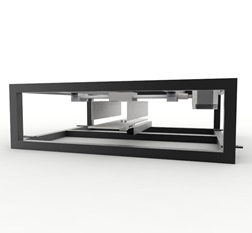
\includegraphics[scale=0.9]{figuras/estrutura/1-Modulo-de-selecao-e-pesagem-de-garrafas.png}
	\caption{Módulo de seleção e pesagem de garrafas}
\end{figure}

\newpage

Primeiramente foi produzido a estrutura em aço 1020 tubular de perfil quadrado (30x30x1,5mm), chapa 16 (Anexo 18), que suporta todos os componentes do módulo. A escolha desse material se deu pela necessidade de uma estrutura sólida, que sofrerá com vibrações geradas no módulo de trituração, e principalmente pelo custo. Como foi utilizado esse material para o módulo de integração, comprar em uma maior quantidade e utilizar entre outros módulos se tornou mais atrativo do que variar a estrutura com materiais diferentes. Com o desenho em CAD, solicitou-se os orçamentos e produziu-se a estrutura, utilizando o processo de fabricação de soldagem com eletrodo revestido, conforme os desenhos técnicos em anexo (Anexos 1) e a figura a seguir:

\begin{figure}[!h]
	\centering
		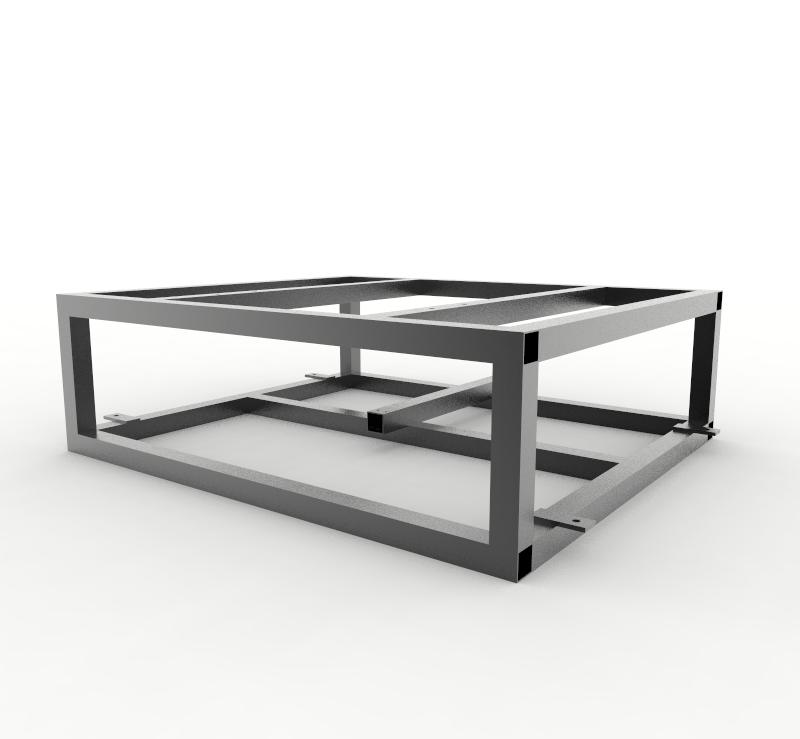
\includegraphics[scale=0.4]{figuras/estrutura/2-Estrutura-do-Modulo-de-selecao.jpg}
	\caption{Estrutura  do Módulo de seleção e pesagem de garrafas}
\end{figure}

A célula de carga foi fixada em um de seus extremos, por parafusos allen M6, porcas e arruelas, na barra centralizada da estrutura. Para seu correto funcionamento, ela deve ser fixada em balanço, de forma que seu extremo sensitivo possa fletir com um aumento de carga. Nesse extremo, fixou-se uma chapa de 1,5 mm, espaçada do seletor por porcas e arruelas, de forma a manter a chapa a uma distância suficiente para receber o peso das garrafas sem tocar em outras partes da estrutura ou no outro extremo da célula de carga. Utilizou-se, por fim, uma peça de PVC (policloreto de polivinila) na superfície da chapa, com o intuito de mantê-la lisa e levemente inclinada. Essa inclinação se fez necessária para que as garrafas inseridas pelo usuário rolem e toquem os sensores capacitivos, utilizados pela eletrônica para identificar o material das garrafas.

\begin{figure}[!h]
	\centering
		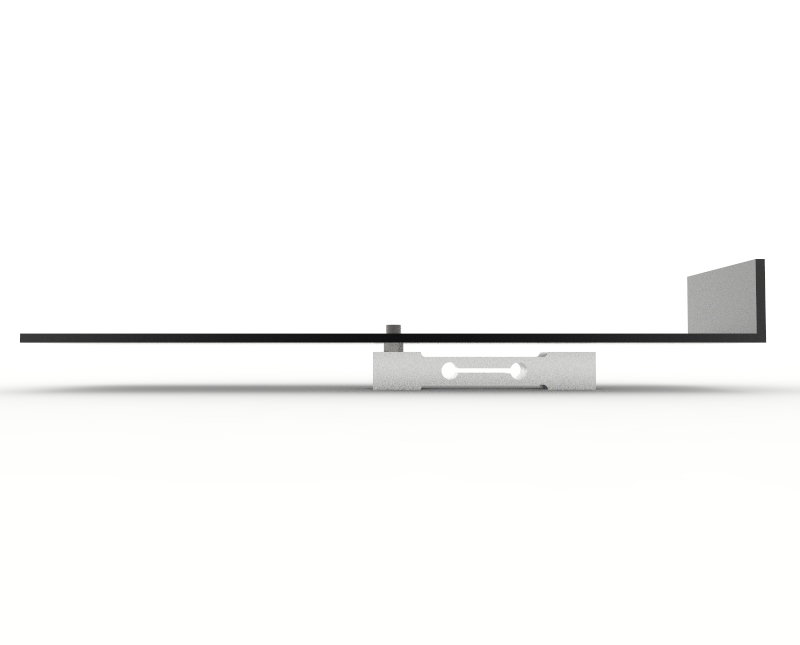
\includegraphics[scale=0.3]{figuras/estrutura/3-Sistema-de-pesagem1.jpg}
	\caption{Sistema de Pesagem}
\end{figure}

\begin{figure}[!h]
	\centering
		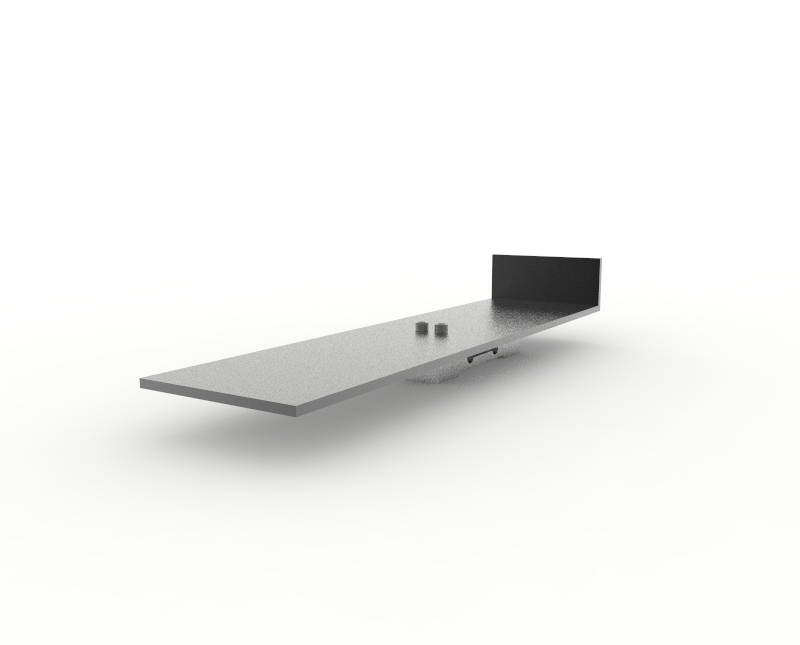
\includegraphics[scale=0.3]{figuras/estrutura/3-Sistema-de-pesagem2.jpg}
	\caption{Sistema de Pesagem}
\end{figure}

O mecanismo direcionador de garrafas foi projetado no modelo de mesas lineares, formado por: uma guia linear de 500mm; dois suportes para guias lineares SK12; um fuso trapezoidal TR8, passo de 8mm, com flange; 2 mancais KP08; um rolamento linear SC12uu; dois pillow blocks, sendo um montado com o rolamento linear e outro com a flange do fuso;  um motor de passo NEMA 17; um acoplamento flexível para eixos de 5mm (saída do motor) e 8mm (fuso); Suporte para motor NEMA 17.

\begin{figure}[!h]
	\centering
		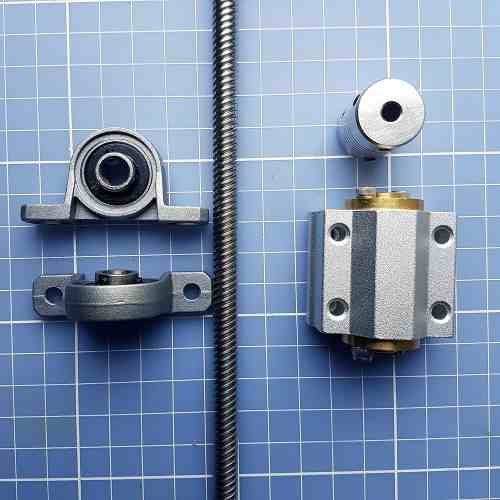
\includegraphics[scale=0.2]{figuras/estrutura/4-Mancais-fuso-acoplamento-pillow.jpg}
	\caption{Mancais, fuso, acoplamento e pillow block com flange}
\end{figure}

\begin{figure}[!h]
	\centering
		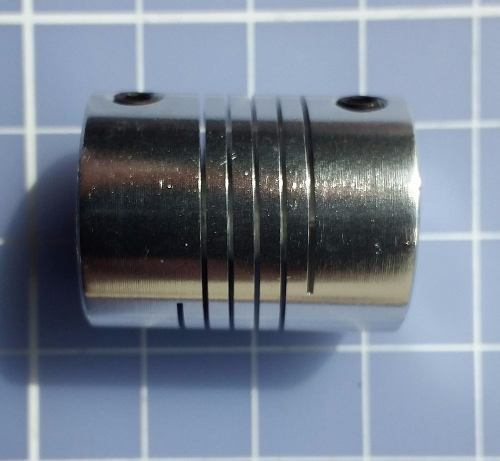
\includegraphics[scale=0.2]{figuras/estrutura/5-Acoplamento-flexivel.jpg}
	\caption{Acoplamento flexivel}
\end{figure}

\begin{figure}[!h]
	\centering
		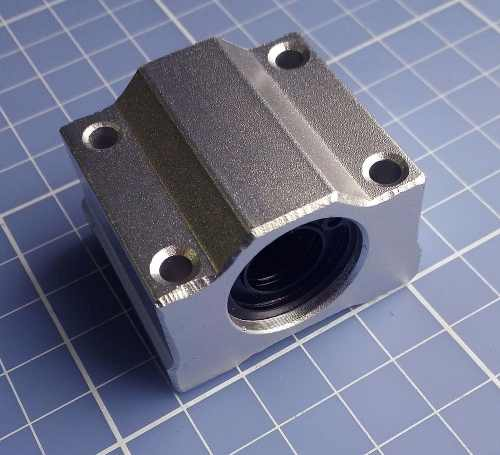
\includegraphics[scale=0.2]{figuras/estrutura/6-Pillow-block-com-rolamento-linear.jpg}
	\caption{Pillow block com rolamento linear}
\end{figure}

\begin{figure}[!h]
	\centering
		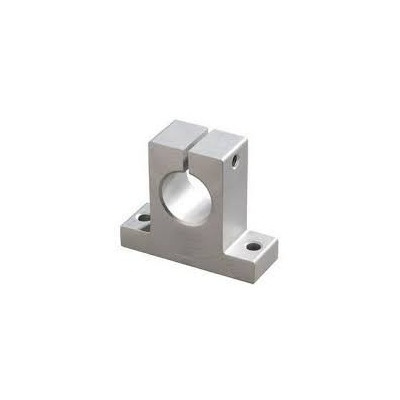
\includegraphics[scale=0.3]{figuras/estrutura/7-Suporte-para-guia-linear.jpg}
	\caption{Suporte para guia linear}
\end{figure}

\begin{figure}[!h]
	\centering
		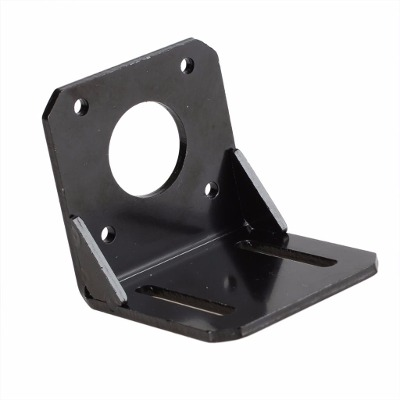
\includegraphics[scale=0.2]{figuras/estrutura/8-Suporte-para-motor-NEMA-17.jpg}
	\caption{Suporte para motor NEMA 17}
\end{figure}

Reutilizou-se para a concepção da garra, que irá envolver as garrafas inseridas no sistema e movê-las para seu respectivo destino, partes de estruturas de CPU’s encontradas em um galpão de armazenamento de lixo do SLU (sistema de limpeza Urbana). Na garra, furou-se uma de suas laterais para encaixe dos sensores capacitivos utilizados pela eletrônica.

\begin{figure}[!h]
	\centering
		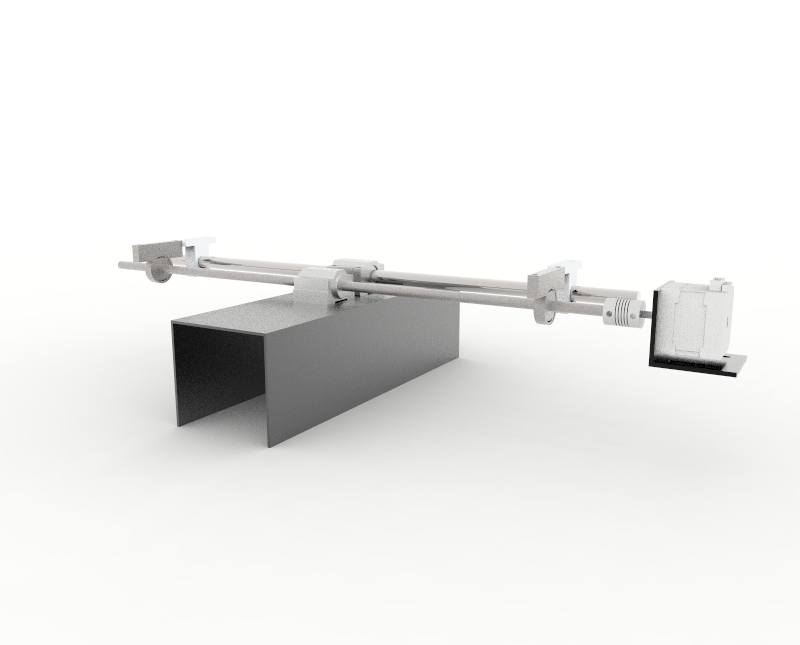
\includegraphics[scale=0.4]{figuras/estrutura/9-Sistema-de-selecao-montado.jpg}
	\caption{Sistema de seleção montado}
\end{figure}

Foram necessários 48 horas de trabalho para concepção do módulo seleção e pesagem, desde o projeto em CAD até o resultado final, de pintura e montagem. A seguir é possível ver imagens das etapas de produção e resultado final deste módulo

\begin{figure}[!h]
	\centering
		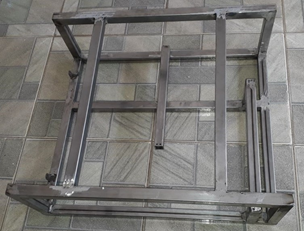
\includegraphics[scale=1.1]{figuras/estrutura/10-Estrutura-do-modulo-de-selecao-e-pesagem-de-garrafas-montado.png}
	\caption{Estrutura do módulo de seleção e pesagem de garrafas montado}
\end{figure}

\begin{figure}[!h]
	\centering
		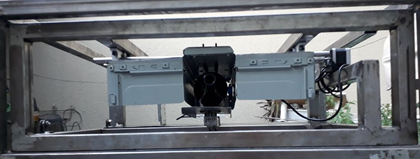
\includegraphics[scale=0.8]{figuras/estrutura/11.png}
	\caption{Modulo de selecao e pesagem de garrafas montado na estrutura de integracao}
\end{figure}

\begin{figure}[!h]
	\centering
		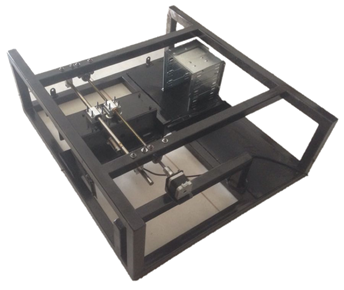
\includegraphics[scale=0.8]{figuras/estrutura/12.png}
	\caption{Módulo de seleção e pesagem de garrafas acabado}
\end{figure}

\subsubsection{Módulo de trituração de embalagens PET}
O módulo de trituração de embalagens PET consiste em um triturador, um funil, uma redução, um motor, uma base para suporte do conjunto e uma gaveta, para armazenamento do plástico triturado. Tanto o motor como a redução foram doadas para o projeto pela Universidade de Brasília (UnB). Todas as outras partes foram produzidas pelos integrantes de estrutura.

\begin{figure}[!h]
	\centering
		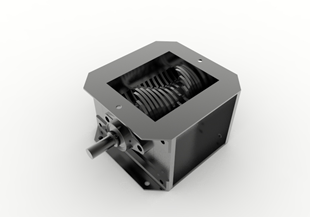
\includegraphics[scale=1.1]{figuras/estrutura/13(1).png}
	\caption{Protótipo do triturador e funil (1)}
\end{figure}

\begin{figure}[!h]
	\centering
		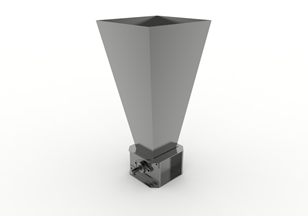
\includegraphics[scale=0.9]{figuras/estrutura/13(2).png}
	\caption{Protótipo do triturador e funil (2)}
\end{figure}

O triturador de plástico a ser utilizado neste projeto foi dimensionado e utilizou-se como base trituradores disponíveis no mercado e projetos open source disponibilizados na internet. Após análise do projeto e aprovação, algumas peças foram usinadas em uma CNC de corte à plasma e retrabalhadas com o intuito de alcançar o melhor acabamento possível. Idealmente, um aço mais duro e apropriado para ferramentas de corte, como aços inoxidáveis ou AISI 1045, seriam utilizados na concepção do triturador. Todavia, para este projeto, as peças usinadas foram de aço AISI 1020, por questões de custo.  O triturador ainda funcionará de maneira satisfatória para o protótipo proposto. Os desenhos técnicos das partes do triturador e sua montagem podem ser vistos nos anexos 2 a 14 , ao final deste trabalho.

Para a concepção do módulo de trituração foram utilizados os seguintes materiais:

\newpage

\begin{table}[!h]
    \centering
    \caption{Materiais módulo de trituração}
    \label{my-label}
    \begin{tabular}{|p{0.15\linewidth}|p{0.15\linewidth}|p{0.15\linewidth}|p{0.15\linewidth}|p{0.15\linewidth}|}
    \hline
    \textbf{Descrição}              & \textbf{Quantidade} & \textbf{Especificação}                                            & \textbf{Material}                                     & \textbf{Processo envolvido}                    \\ \hline
    Chapa                           & 1                   & 3mm de espessura                                                  & Aço AISI 1020                                         & Usinado à Plasma                               \\ \hline
    Chapa                           & 1                   & 5mm de espessura                                                  & Aço AISI 1020                                         & Usinado à Plasma                               \\ \hline
    Chapa                           & 1                   & 6mm de espessura                                                  & Aço AISI 1020                                         & Usinado à Plasma                               \\ \hline
    Barra Sextavada                 & 1                   & 25,4mm de altura                                                  & Aço AISI 1020                                         & Pontas usinadas em torno                       \\ \hline
    Motor                           & 1                   & 1 HP                                                              & -                                                     & -                                              \\ \hline
    Acoplamento, Flexível, Elástico & 2 pares             &                                                                   & Ferro fundido, com elemento de sacrifício em plástico & Furos usinados em torno e furadeira de bancada \\ \hline
    Barra de chaveta                & 1                   & 6x6x500 mm                                                        & Aço                                                   & Usinagem em CNC                                \\ \hline
    Moscas                          & 6                   & M6                                                                & Aço                                                   & -                                              \\ \hline
    Mancais com rolamento           & 2                   & UCFL 204                                                          & Mancal em ferro fundido                               & -                                              \\ \hline
    Tubo Perfilado Quadrado         & 9 metros            & \begin{tabular}[c]{@{}c@{}}30x30x1,5mm\\ \\ Chapa 16\end{tabular} & Aço AISI 1020                                         & Soldagem                                       \\ \hline
    Chapa                           & 1                   & 100x100x4 mm                                                      & Aço AISI 1020                                         & -                                              \\ \hline
    Chapa                           & 1                   & 275x183x20 mm                                                     & Madeira MDF                                           & -                                              \\ \hline
    Redutor                         & 1                   & 1:40                                                              & -                                                     & -                                              \\ \hline
    \end{tabular}
\end{table}

Sendo um dos módulos mais complexos e que demanda mais tempo para conclusão desse trabalho, optou-se por produzi-lo ao mesmo tempo em que as outras etapas fossem realizadas. Até o momento, foram empregados 328 horas de trabalho, divididos em etapas. Primeiramente, orçou-se a produção de todas as peças para o triturador, que foram usinadas à plasma. A partir daí, os integrantes ficaram responsáveis por dar o acabamento nessas peças, com o uso de esmerilhadeira e flaps de granulações destintas, e produzir as outras partes que poderiam ser feitas no galpão. 

\newpage

\begin{figure}[!h]
	\centering
		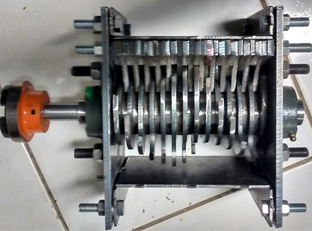
\includegraphics[scale=0.7]{figuras/estrutura/14.png}
	\caption{Triturador apos todas as etapas}
\end{figure}

Com o uso do torno, usinou-se o eixo sextavado e arruelas, conforme as dimensões demonstradas no anexo 4 . Com o uso da furadeira de bancada, se deu o acabamento nos furos para fixação por parafusos, porcas e arruelas. Durante todos esses processos, a montagem era refeita para nova calibração do triturador, até o ponto no qual as facas móveis rotacionassem sem grande esforço.

\begin{figure}[!h]
	\centering
		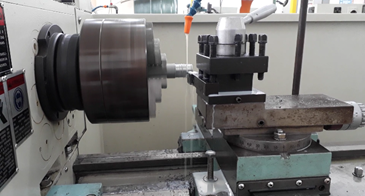
\includegraphics[scale=0.7]{figuras/estrutura/15.png}
	\caption{Usinagem do eixo}
\end{figure}

O redutor utilizado neste módulo é do tipo coroa e rosca sem-fim da WEG-CESTARI, modelo MAGMA-K, redução nominal de 40, tamanho 4, projetado para acionamento de toda classe de máquinas e equipamentos de baixa velocidade. A redução de rotação do motor, 1700 rpm, é necessária para o correto funcionamento do triturador. Com a redução, é possível atingir maior torque na entrada do triturador, suficiente para cortar plástico. Além disso, uma rotação mais baixa garante uma menor temperatura na região de trituração. 

\begin{figure}[!h]
	\centering
		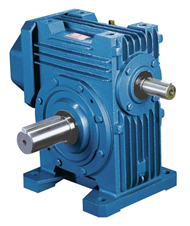
\includegraphics[scale=0.6]{figuras/estrutura/16.png}
	\caption{Redutor WEG-CESTARI MAGMA-K}
\end{figure}

No anexo 15, é possível ver a potência de entrada e de saída, o momento de torção de saída, a carga radial de saída, o rendimento e a redução efetiva do modelo utilizado neste trabalho.

Para fazer a conexão e a correta transmissão de rotação entre motor, redutor e o triturador, foram utilizados 2 pares de acoplamentos em ferro fundido. Eles são acoplamentos flexíveis e torcionalmente elásticos, com elementos de sacrifício elásticos em poliuretano resistente à poeira, água, óleo e intempéries. As corretas dimensões e especificações dos acoplamentos podem ser vistas no anexo 16.

\begin{figure}[!h]
	\centering
		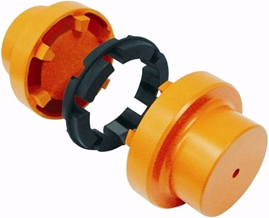
\includegraphics[scale=0.6]{figuras/estrutura/17.png}
	\caption{Acoplamento flexível elástico}
\end{figure}

\begin{figure}[!h]
	\centering
		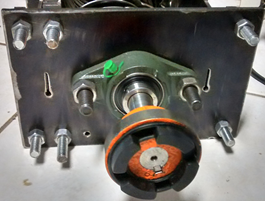
\includegraphics[scale=0.6]{figuras/estrutura/18(1).png}
	\caption{Eixos com acoplamentos flexíveis, chavetas e moscas (1)}
\end{figure}

Esses acoplamentos admitem desalinhamentos radiais, axiais e angulares entre os eixos acoplados e ainda absorve choques e vibrações provenientes da máquina movida ou motora. Tendo construção simplificada, permite instalação rápida e segura, dispensando lubrificação e minimizando a manutenção. O modelo ideal seria o TAMANHO 97, capaz de suportar o momento torsor atuante para vida infinita conforme o catálogo do anexo 16, porém foi utilizado o TAMANHO 50 que atende as necessidades do protótipo. Fornecidos com construção sem furação, foram necessárias a usinagem para encaixe nos eixos, dos rasgos de chaveta e de furos  para fixação por moscas. Para os eixos de saída do motor e de entrada do redutor, utilizou-se apenas de moscas para a fixação dos acoplamentos, uma vez que a rotação nesses eixos são altas e o torque baixo. Para os eixos de saída do redutor e de entrada do triturador, além dos moscas, utilizou-se das chavetas, para melhor fixação dos acoplamentos e correta transmissão do torque gerado.  

\newpage

\begin{figure}[!h]
	\centering
		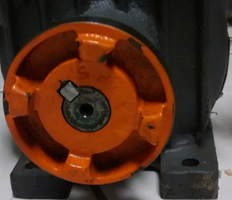
\includegraphics[scale=0.6]{figuras/estrutura/18(2).png}
	\caption{Eixos com acoplamentos flexíveis, chavetas e moscas (2)}
\end{figure}

Por fim, produziu-se a base para o sistema de trituração. Feita em aço 1020 tubular de perfil retangular (20x30x1,5 mm), chapa 16 (anexo 17), essa estrutura tinha 2 objetivos principais. Primeiramente, manter o maior alinhamento e nivelamento possível entre os eixos do motor, do redutor e do triturador. Além disso, é nela que se acopla o compartimento de armazenamento das garrafas PET após a trituração.

\begin{figure}[!h]
	\centering
		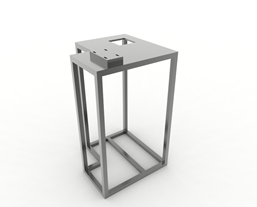
\includegraphics[scale=1.1]{figuras/estrutura/19.png}
	\caption{Estrutura do módulo de trituração}
\end{figure}

Após todo o projeto e produção deste módulo, seguiu-se para a montagem final. É importante salientar que procurou-se manter os eixos coincidentes, para diminuir os esforços do motor, redutor e triturador e garantir um melhor funcionamento.

\begin{figure}[!h]
	\centering
		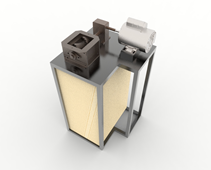
\includegraphics[scale=1.1]{figuras/estrutura/20(1).png}
	\caption{Projeto completo do módulo de trituração}
\end{figure}

\subsubsubsection{Cálculo do torque necessário no triturador}
Para encontrar a força necessária em que o polímero se rompa mesmo nas condições mais difíceis, o cálculo parte de onde a garrafa PET apresenta a seção mais espessa, que é o gargalo próximo ao bocal da tampa, como ilustra a Figura 33 e 34. Temos o diâmetro externo e interno de 25 mm e 22 mm respectivamente, assim conseguimos calcular a área da seção.

\begin{figure}[!h]
	\centering
		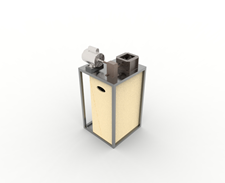
\includegraphics[scale=1.2]{figuras/estrutura/20(2).png}
	\caption{Projeto completo do módulo de trituração}
\end{figure}

\begin{figure}[!h]
	\centering
		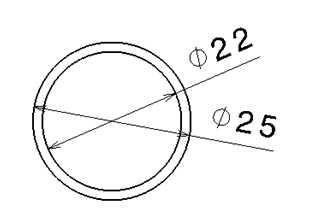
\includegraphics[scale=0.7]{figuras/estrutura/21(1).png}
	\caption{Seção próxima ao bocal e Garrafa PET}
\end{figure}

\begin{figure}[!h]
	\centering
		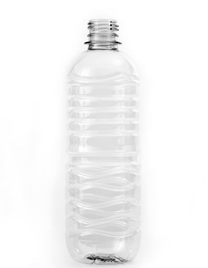
\includegraphics[scale=0.6]{figuras/estrutura/21(2).png}
	\caption{Seção próxima ao bocal e Garrafa PET}
\end{figure}

\begin{equation}
    A = \frac{\Pi \ast (D^{2}- d^{2})}{4}
\end{equation}

\begin{equation}
    A = \frac{\Pi \ast (0,025^{2}- 0,022^{2})}{4}
\end{equation}

\begin{equation}
    A = 1,107 \ast 10^{-4} \ast m^{2}
\end{equation}

Partindo da área da seção da garrafa calculada acima e da tensão de ruptura do PET de 25 MPa, calcula-se a carga aplicada necessária para romper o material.

\begin{equation}
    F = \tau rup \ast A
\end{equation}

\begin{equation}
    F = 25.10^{6}. 1,107.10^{-4}
\end{equation}

\begin{equation}
    F = 2768,53 N
\end{equation}

Com a força definida e o braço de alavanca de 6 cm da faca do triturador chegamos ao valor de 166,11 Nm de torque necessários para cortar a garrafa PET. A entrega do motor disponível é de 736 W e 28,33 Hz atuando junto com uma redução de 1:40 que proporciona o torque de 165,39 Nm, que apesar de não suprir totalmente a demanda chega muito próximo do necessário, o que para um protótipo é satisfatório.

\begin{equation}
    P = 2 \ast \Pi \ast f \ast Tmotor
\end{equation}

\begin{equation}
    736 = 2 \ast \Pi \ast 28,33 \ast Tmotor
\end{equation}

\begin{equation}
    Tmotor = 4,13 Nm
\end{equation}

\begin{equation}
    Tredutor = Tmotor \ast 40
\end{equation}

\begin{equation}
    Tredutor = 165,39 Nm
\end{equation}

O eixo do triturador possui seu menor diâmetro de 20 mm, que se mostrou capaz de resistir ao momento torsor atuante, com tensões de cisalhamento bem abaixo do limite de escoamento de 380 MPa para o aço AISI 1020.

\begin{equation}
    \tau = \frac{T \ast c}{J}
\end{equation}

\begin{equation}
    \tau = \frac{166,11 \ast 0,01}{1,57 \ast 10^{-8}}
\end{equation}

\begin{equation}
    \tau = 105,80 MPa
\end{equation}

\subsubsubsection{Compartimentos de armazenamento}
Os compartimentos de armazenamento serão dimensionados de acordo com a natureza da garrafa, bem como parâmetros de operação dos subsistemas (trituração, seleção, leitura de produto, etc) e custo para manufatura.

Para o plástico PET triturado, o compartimento será desenvolvido em madeira MDF no formato de gaveta, de acordo com as dimensões estruturais da máquina.


\begin{figure}[!h]
	\centering
		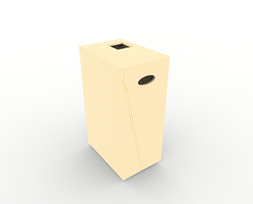
\includegraphics[scale=1.2]{figuras/estrutura/22.png}
	\caption{Compartimento de armazenamento de plástico triturado}
\end{figure}

Também em madeira MDF, serão as canaletas do compartimento de armazenamento de garrafas de vidro, que terão o intuito de guiar as garrafas até o fundo do compartimento sem a ocorrência de ruptura do material. Para tal, as canaletas possuirão uma angulação e batentes. 

\begin{figure}[!h]
	\centering
		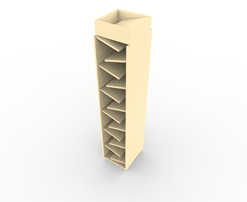
\includegraphics[scale=1.2]{figuras/estrutura/23.png}
	\caption{Compartimento de armazenamento de garrafas de vidro}
\end{figure}

Para garantir o pleno funcionamento, haverá uma porta de acesso em cada compartimento para o recolhimento dos resíduos e de limpeza dos compartimentos.

\subsubsubsection{Dimensionamento do Compartimento de Garrafas PET}
No dimensionamento do compartimento de garrafas PET, o principal parâmetro é o volume que será guardado na gaveta. Primeiramente sabe-se que a densidade do PET é de 1,38 gramas por cm cubico, e que uma garrafa PET 600ml comumente encontrada no mercado possui cerca de 25g. Para este protótipo, tomaremos 50 garrafas PET de 600 ml como capacidade máxima. Portanto:

\begin{equation}
    m = 50 \ast 25 = 1.250 g
\end{equation}

Já o volume total será de:

\begin{equation}
    V = \frac{m}{\rho} = 905,80 cm^{3}
\end{equation}

Assim as dimensões da gaveta terão que garantir no mínimo um espaço de armazenamento de 905,80 cm cubicos. Entretanto esse valor, não considera os espaços vazios entre os granulados, sendo necessário uma medida experimental do volume de uma garrafa triturada.

\subsubsubsection{Dimensionamento do Compartimento de Garrafas de Vidro}
Para o compartimento de armazenamento de garrafas de vidro o primeiro cálculo para o dimensionamento é a inclinação máxima da superfície de rolamento da garrafa. Para este cálculo é necessário o valor da tenacidade à fratura KIC,min do vidro (0,62 MPa.m1/2 ) e o módulo de Young (66,3 GPa), dessa forma podemos encontrar a tenacidade do material Gc, através da seguinte relação:

\begin{equation}
    G_{c} = \frac{K_{ic}^{2}}{E} = \frac{0,62^{2}}{66,3} = 5,80 \frac{kj}{m^{2}}
\end{equation}

A tenacidade Gc é a propriedade que quantifica a energia por unidade de área necessária para que o material falhe. Assumindo uma garrafa com as seguintes dimensões:

\newpage

\begin{figure}[!h]
	\centering
		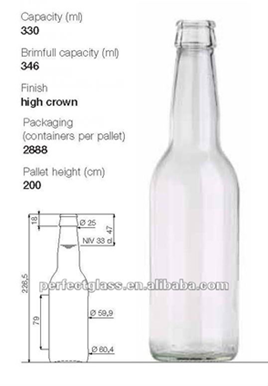
\includegraphics[scale=0.8]{figuras/estrutura/24.png}
	\caption{Garrafa Long Neck}
\end{figure}

\begin{figure}[!h]
	\centering
		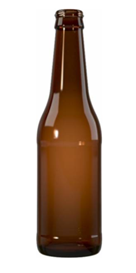
\includegraphics[scale=0.7]{figuras/estrutura/25.png}
	\caption{Garrafa Long Neck}
\end{figure}

\begin{itemize}
    \item Cor: Âmbar
    \item Material: vidro
    \item Gargalo: Twist Off
    \item Dimensão: 6,16 X 22,7 cm
    \item Diâmetro: 6,16 cm
    \item Altura: 22,7 cm
    \item Peso: 190g
    \item Volume útil: 355ml
    \item Volume Total: 275ml
    \item Qtde. Caixa: 24 unidades
    \item Dimensão do Pallet: 1.00 x 1.20 X 2.46m
    \item Peso Pallet: 700 kg
\end{itemize}

Foi efetuado um desenho aproximado no software Catia V5R19, onde é possível obter o valores mais exatos das propriedades geométricas.

\begin{figure}[!h]
	\centering
		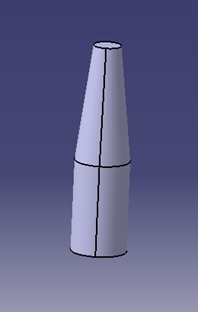
\includegraphics[scale=0.7]{figuras/estrutura/26.png}
	\caption{CAD aproximado da garrafa}
\end{figure}

\begin{figure}[!h]
	\centering
		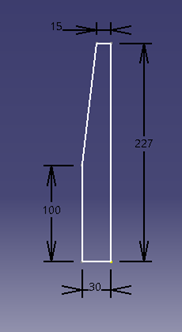
\includegraphics[scale=0.7]{figuras/estrutura/27.png}
	\caption{CAD garra, dimensões em mm}
\end{figure}

Assumindo uma garrafa com espessura de 3mm, a área de secção transversal que estará em contato com o plano inclinado será de 537,21 mm2 é possível encontrar o valor da energia de ruptura J.

\begin{equation}
    J_{rup} = G_{c} \ast A = 3,116 Joules
\end{equation}

Da dinâmica da garrafa, seu movimento de rolamento ocorrerá através de diversos planos inclinados. Assumindo que a primeira iteração a garrafa partirá com uma velocidade inicial negligenciável, devido ao controle do motor de passo presente no mecanismo de seleção de garrafas do protótipo, podemos assumir calcular diferença de altura através da equação de energia potencial:

\begin{equation}
    E_{potencial} = mg\Delta z
\end{equation}

Assim, podemos determinar a altura mínima na qual o vidro falhará:

\begin{equation}
    \Delta z = \frac{J_{rup}}{mg} = \frac{3,116}{0,190 \ast 9,81} = 1,6717 m
\end{equation}

O compartimento terá uma largura interna de aproximadamente 17 cm, através de uma relação trigonométrica podemos calcular a inclinação máxima:

\begin{equation}
    \Theta _{max,1} = \tan^{-1}\frac{\Delta z}{L} = \tan^{-1}\frac{167,17}{17} = 84,19 graus
\end{equation}

Introduzindo um fator de segurança FS de 25\% na altura mínima, recalculamos o valor da inclinação máxima:

\begin{equation}
    \Theta _{max,2} = \tan^{-1}\frac{\Delta z \ast FS}{L} = \tan^{-1}\frac{125,38}{17} = 82,23 graus
\end{equation}

Portanto a garrafa não falhará para inclinações menores que 82,23 graus.

\subsubsubsection{Módulo de Integração}
O módulo de integração foi pensado com o intuito de receber todos os componentes e módulos desenvolvidos nesse projeto. Além disso, ele será a interface física entre o usuário e a máquina. Portanto, ela também foi pensado para garantir segurança, acessibilidade e visibilidade dentro do ambiente de uso. A figura à seguir ilustra como é o projeto do módulo de integração.

\begin{figure}[!h]
	\centering
		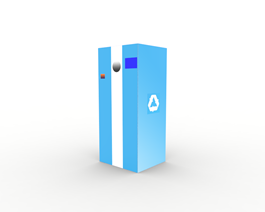
\includegraphics[scale=1.2]{figuras/estrutura/28.png}
	\caption{Protótipo da estação coletora}
\end{figure}

Suas dimensões foram definidas com base em alguns pontos que deveriam ser levados em consideração: 

\begin{itemize}
    \item Dificultar o acesso de crianças ao interior da máquina;
    \item Manter uma posição confortável ao usuário, que deverá ter acesso à entrada de garrafas, ao leitor de QRcode e a tela de interação;
    \item Volume suficiente para armazenar todos os módulos, componentes e garrafas no seu interior;
\end{itemize}

Ao final de toda a simulação em CAD, com todos os módulos e com o uso do ambiente Human Builder do software CATIA V5, definiu-se as dimensões da estrutura em 1,80 metros de altura, 80 centímetros de comprimento e 70 centímetros de largura. O protótipo simulado e o produzido da estrutura base do módulo de integração podem ser vistos nas imagens a seguir:

\begin{figure}[!h]
	\centering
		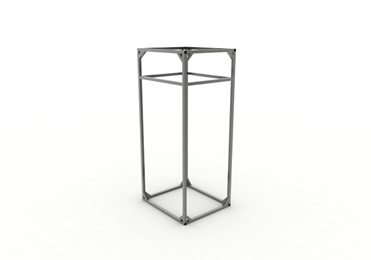
\includegraphics[scale=1.0]{figuras/estrutura/29.png}
	\caption{Simulação da Estrutura Tubular do Módulo de Integração}
\end{figure}

\begin{figure}[!h]
	\centering
		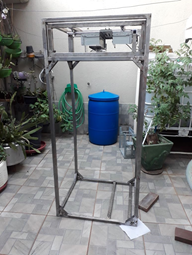
\includegraphics[scale=1.1]{figuras/estrutura/30.png}
	\caption{Estrutura Tubular do Módulo de Integração finalizada}
\end{figure}

A estrutura é composta por uma gaiola de aço AISI 1020 tubular de perfil quadrado (30x30x1,5mm), chapa 16, que funciona como armação  principal. Esse material foi selecionado porque, além da confiabilidade, suas propriedades mecânicas atendem as necessidades do projeto, garantindo uma estrutura sólida. Os desenhos técnicos da estrutura podem ser vistos nos anexos desse trabalho. 

Placas de zinco foram escolhidas para fechar toda a estrutura por ser um material de baixo custo, além de ser um material de alta manuseabilidade, tornando o processo de fixação na armação principal simples e suficiente. Serão feitos furos para a fixação de todos os componentes que precisam ter o acesso do usuário. 

\subsubsection{Integração entre módulos}
Ao final dos processos de produção de cada módulo até aqui, realizou-se a integração entre as partes para a garantia do funcionamento da máquina ao final do projeto. Alguns resultados dessa integração podem ser vistos a seguir:

\begin{figure}[!h]
	\centering
		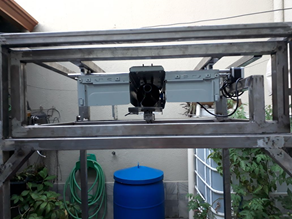
\includegraphics[scale=1.1]{figuras/estrutura/31.png}
	\caption{Encaixe do modulo de seleção}
\end{figure}

\newpage

\begin{figure}[!h]
	\centering
		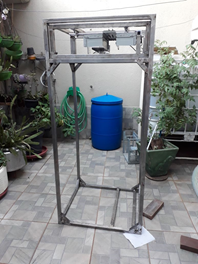
\includegraphics[scale=1.2]{figuras/estrutura/32.png}
	\caption{Módulo de integração com modulo de seleção integrados}
\end{figure}

\subsubsection{Integração entre módulos}

Alguns testes foram ou serão realizados para garantia do correto funcionamento da máquina como um todo.
\begin{itemize}
    \item Teste para tempo médio de trituração do plástico. 
    \item Experimentos para avaliar a eficácia do armazenamento das garrafas de vidro.
    \item Análises computacionais, utilizando CATIA V5 ou ANSYS 18.1, para validação do design e da estrutura, de forma a garantir correta integração entre os sistemas e correto dimensionamento para suportar os esforços e vibrações existentes no projeto.
\end{itemize}  
